
The optimal $O(n)$ memory access and low work-complexity allows the SEM
to be implemented with relatively high polynomial orders, with $N=7$ or 8
being typical production values.
%
   Elevated order is of paramount performance for long time integrations (i.e.,
where small scales are propagated over long distances) as noted in early work
on linear transport by by Kreiss and Oliger \cite{kreiss72}.  High-order is
equally important in the case of {\em nonlinear} (i.e., turbulent) transport,
as illustrated in Fig. \ref{fig:sprague}, left.  Here, we see spatial spectra
for velocity at $z=100$m in an atmospheric boundary layer benchmark problem
for $n=256^3$, $512^3$, $1024^3$, and $2048^3$ resolution, along
with the $k^{-\frac{5}{3}}$ spectrum predicted by Kolmogorov theory
\cite{Tomboulides2024ABL}.
We note that the $8$th-order SEM at $256^3$ outperforms 2nd-order finite
volume (FV) discretization at $512^3$.  Moreover, the reduction in spatial
resolution allows the SEM to use a $2\times$ larger timestep, for an overall
reduction of $16\times$ in number of degrees-of-freedom for 8th-order SEM vs.
2nd-order FV at the same accuracy.  As noted in an earlier work \cite{Min2024Wind},
the SEM also outperforms the FV by almost a factor of two in wall-clock time
per grid-point per time-step (Fig. \ref{fig:sprague}, right), so NekRS is well
over an order-of-magnitude faster than traditional FV for this class of
problems.

\begin{figure}[h]
    \centering
    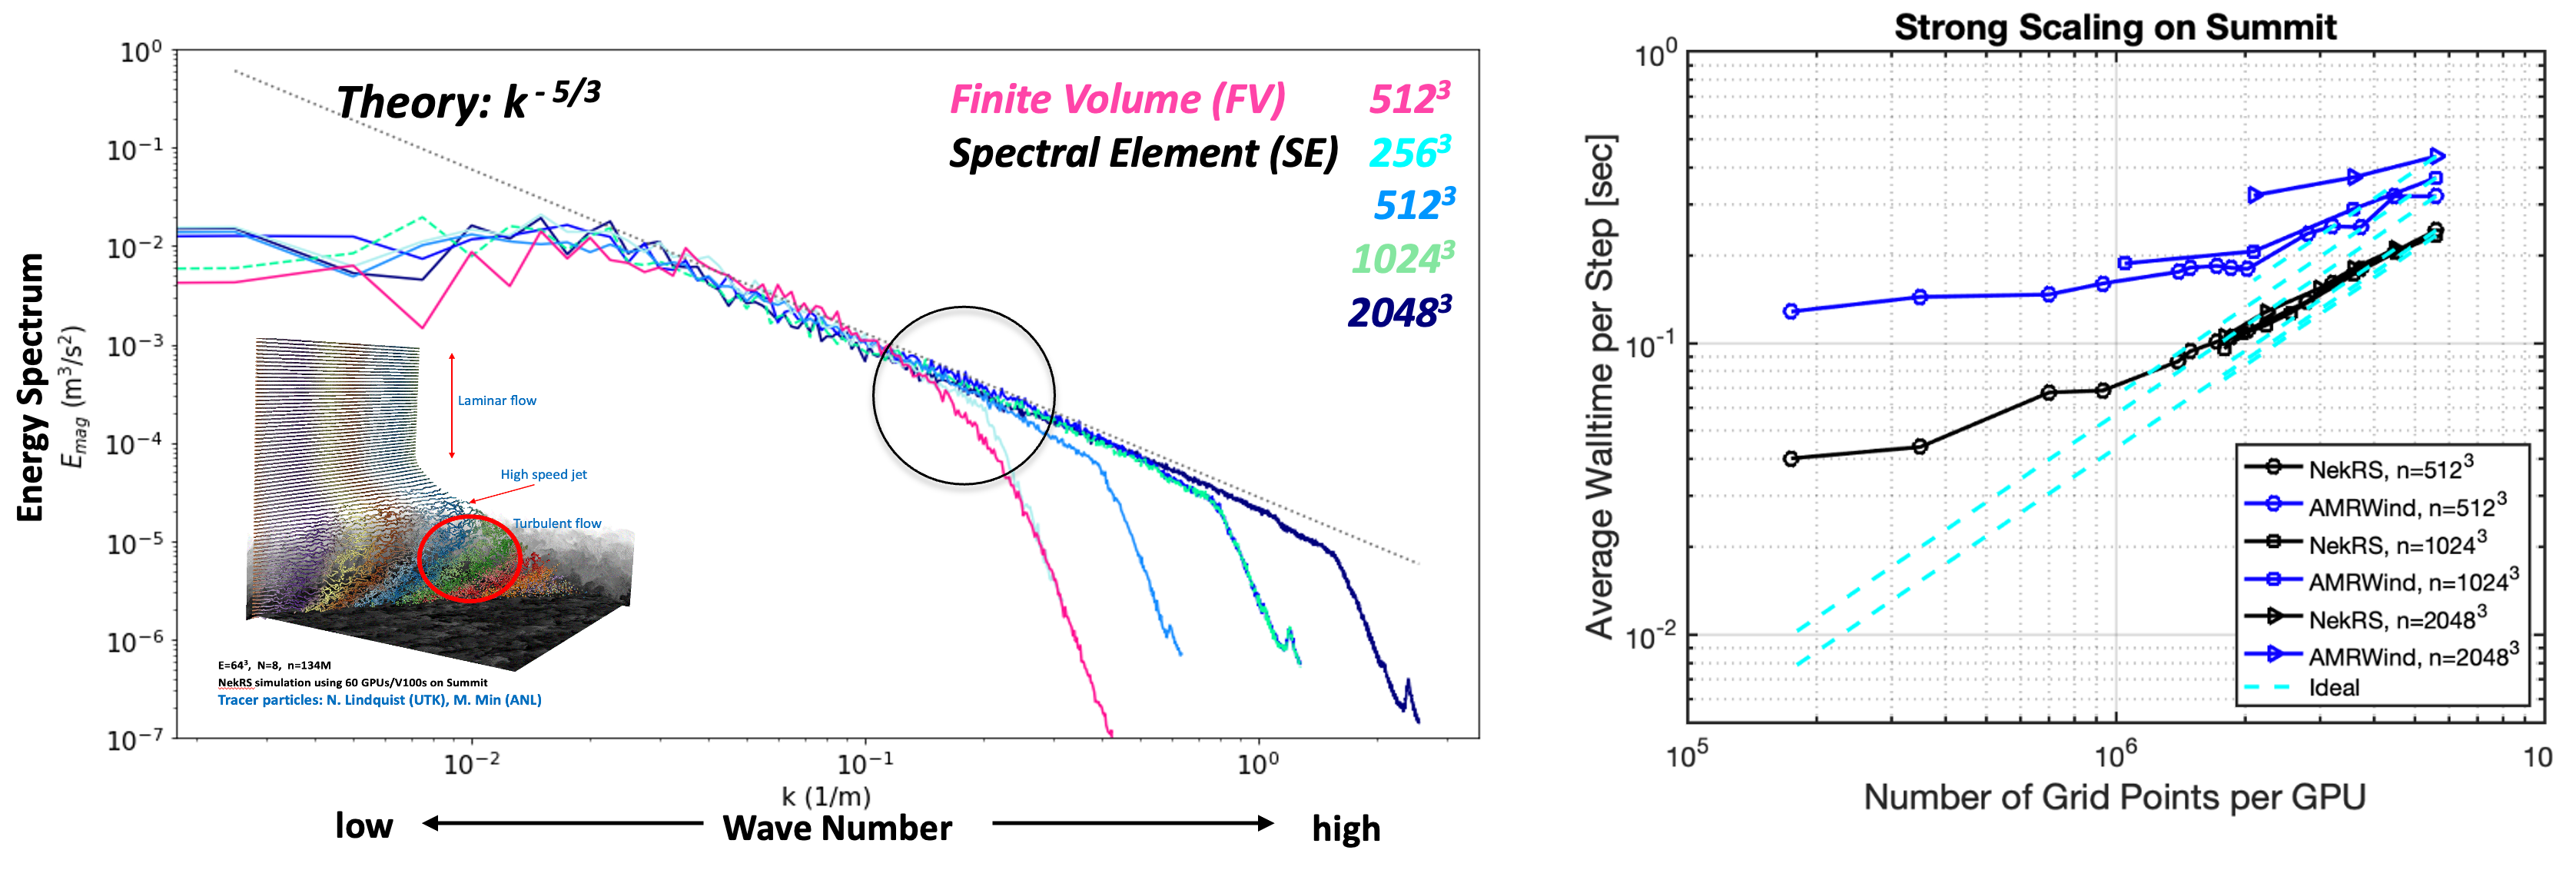
\includegraphics[width=0.98\linewidth]{figs/sprague_energy_spectrum.png}
\caption{
Performance comparison of SEM vs. finite-volume (FV): (left) energy spectra
for $n=256^3$--$2048^3$ for NekRS and $n=512^3$ for FV; 
(right) strong-scaling of SEM (NekRS) vs. FV (AMRWind) on Summit for identical
resolutions and timestep sizes.
}
\label{fig:sprague}
\end{figure}
